\documentclass{standalone}
\usepackage{tikz}
\usetikzlibrary{patterns, positioning}


\begin{document}
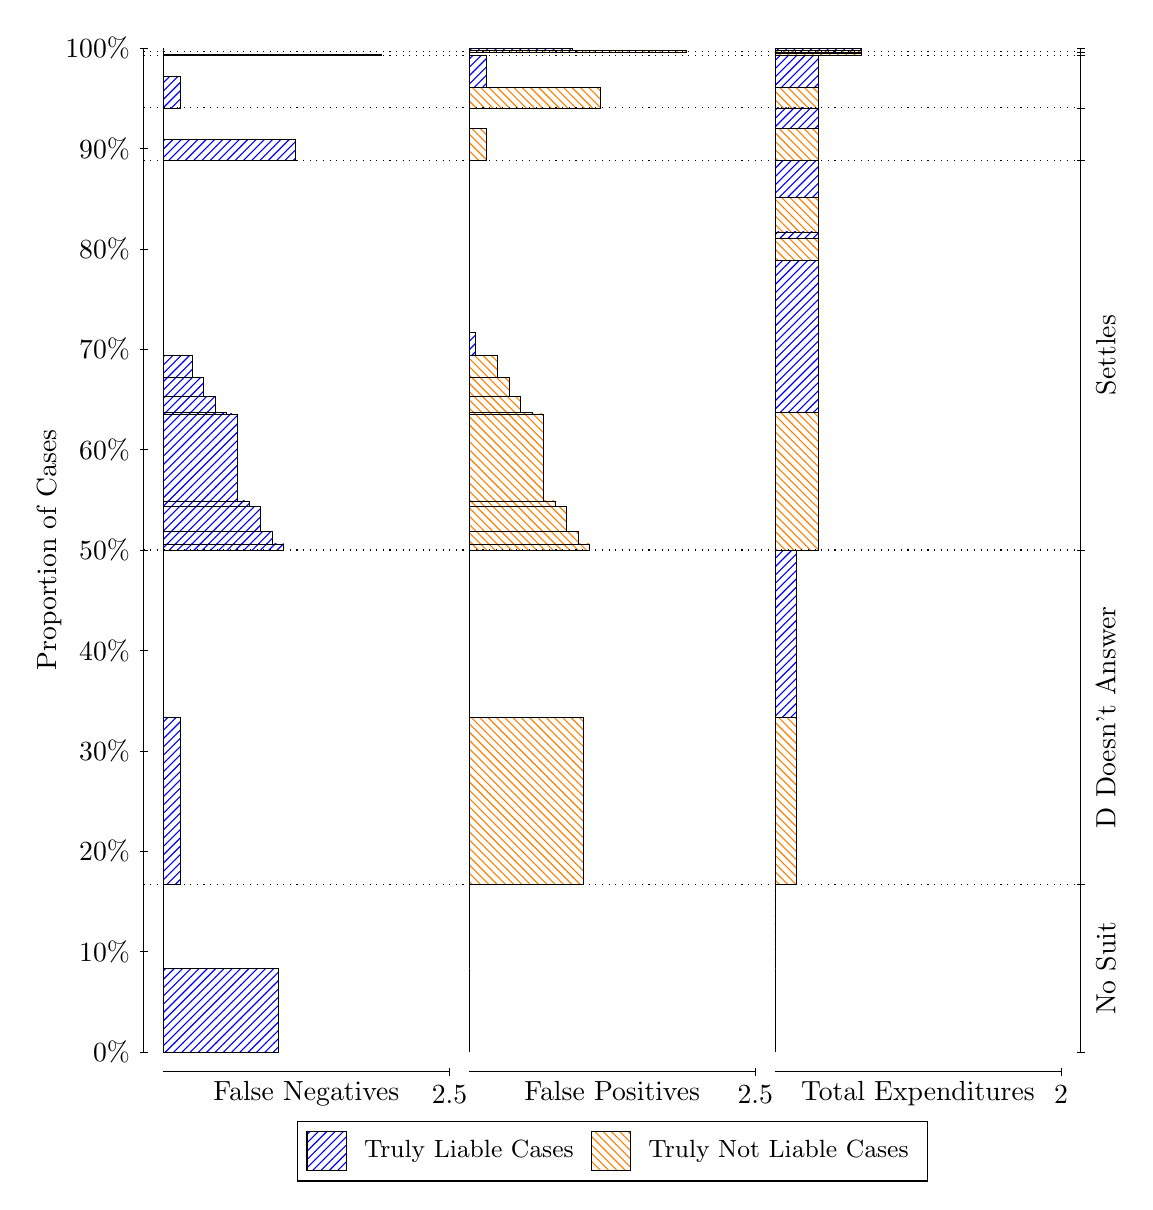
\begin{tikzpicture}
\draw[black, very thin] (1.5,1.75) -- (1.5,14.5);
\node[rotate=90, text=black, anchor=center] at (0.3, 8.125) {Proportion of Cases};
\draw[black, very thin] (1.45,1.75) -- (1.55,1.75);
\node[text=black, anchor=east] at (1.45, 1.75) {0\%};
\draw[black, very thin] (1.45,3.025) -- (1.55,3.025);
\node[text=black, anchor=east] at (1.45, 3.025) {10\%};
\draw[black, very thin] (1.45,4.3) -- (1.55,4.3);
\node[text=black, anchor=east] at (1.45, 4.3) {20\%};
\draw[black, very thin] (1.45,5.575) -- (1.55,5.575);
\node[text=black, anchor=east] at (1.45, 5.575) {30\%};
\draw[black, very thin] (1.45,6.85) -- (1.55,6.85);
\node[text=black, anchor=east] at (1.45, 6.85) {40\%};
\draw[black, very thin] (1.45,8.125) -- (1.55,8.125);
\node[text=black, anchor=east] at (1.45, 8.125) {50\%};
\draw[black, very thin] (1.45,9.4) -- (1.55,9.4);
\node[text=black, anchor=east] at (1.45, 9.4) {60\%};
\draw[black, very thin] (1.45,10.675) -- (1.55,10.675);
\node[text=black, anchor=east] at (1.45, 10.675) {70\%};
\draw[black, very thin] (1.45,11.95) -- (1.55,11.95);
\node[text=black, anchor=east] at (1.45, 11.95) {80\%};
\draw[black, very thin] (1.45,13.225) -- (1.55,13.225);
\node[text=black, anchor=east] at (1.45, 13.225) {90\%};
\draw[black, very thin] (1.45,14.5) -- (1.55,14.5);
\node[text=black, anchor=east] at (1.45, 14.5) {100\%};

\draw[black, very thin] (13.4,1.75) -- (13.4,14.5);
\draw[black, very thin] (13.35,1.75) -- (13.45,1.75);
\node[anchor=west] at (13.35, 1.75) {};
\draw[black, very thin] (13.35,3.875) -- (13.45,3.875);
\node[anchor=west] at (13.35, 3.875) {};
\draw[black, very thin] (13.35,8.125) -- (13.45,8.125);
\node[anchor=west] at (13.35, 8.125) {};
\draw[black, very thin] (13.35,13.077) -- (13.45,13.077);
\node[anchor=west] at (13.35, 13.077) {};
\draw[black, very thin] (13.35,13.74) -- (13.45,13.74);
\node[anchor=west] at (13.35, 13.74) {};
\draw[black, very thin] (13.35,14.404) -- (13.45,14.404);
\node[anchor=west] at (13.35, 14.404) {};
\draw[black, very thin] (13.35,14.452) -- (13.45,14.452);
\node[anchor=west] at (13.35, 14.452) {};
\draw[black, very thin] (13.35,14.5) -- (13.45,14.5);
\node[anchor=west] at (13.35, 14.5) {};

\draw[black, very thin, pattern color=blue, pattern=north east lines] (1.75,1.75) rectangle (3.2033,2.8125);
\draw[black, very thin, pattern color=orange, pattern=north west lines] (1.75,2.8125) rectangle (1.75,3.875);
\draw[black, very thin, pattern color=blue, pattern=north east lines] (1.75,3.875) rectangle (1.968,6);
\draw[black, very thin, pattern color=orange, pattern=north west lines] (1.75,6) rectangle (1.75,8.125);
\draw[black, very thin, pattern color=blue, pattern=north east lines] (1.75,8.125) rectangle (3.276,8.203);
\draw[black, very thin, pattern color=blue, pattern=north east lines] (1.75,8.203) rectangle (3.1307,8.3608);
\draw[black, very thin, pattern color=blue, pattern=north east lines] (1.75,8.3608) rectangle (2.9853,8.6758);
\draw[black, very thin, pattern color=blue, pattern=north east lines] (1.75,8.6758) rectangle (2.84,8.7491);
\draw[black, very thin, pattern color=blue, pattern=north east lines] (1.75,8.7491) rectangle (2.6947,9.8526);
\draw[black, very thin, pattern color=blue, pattern=north east lines] (1.75,9.8526) rectangle (2.5493,9.8769);
\draw[black, very thin, pattern color=blue, pattern=north east lines] (1.75,9.8769) rectangle (2.404,10.078);
\draw[black, very thin, pattern color=blue, pattern=north east lines] (1.75,10.078) rectangle (2.2587,10.316);
\draw[black, very thin, pattern color=blue, pattern=north east lines] (1.75,10.316) rectangle (2.1133,10.601);
\draw[black, very thin, pattern color=orange, pattern=north west lines] (1.75,10.601) rectangle (1.75,13.077);
\draw[black, very thin, pattern color=blue, pattern=north east lines] (1.75,13.077) rectangle (3.4213,13.337);
\draw[black, very thin, pattern color=orange, pattern=north west lines] (1.75,13.337) rectangle (1.75,13.74);
\draw[black, very thin, pattern color=blue, pattern=north east lines] (1.75,13.74) rectangle (1.968,14.143);
\draw[black, very thin, pattern color=orange, pattern=north west lines] (1.75,14.143) rectangle (1.75,14.404);
\draw[black, very thin, pattern color=blue, pattern=north east lines] (1.75,14.404) rectangle (4.5113,14.422);
\draw[black, very thin, pattern color=orange, pattern=north west lines] (1.75,14.422) rectangle (1.75,14.452);
\draw[black, very thin, pattern color=orange, pattern=north west lines] (1.75,14.452) rectangle (1.75,14.47);
\draw[black, very thin, pattern color=blue, pattern=north east lines] (1.75,14.47) rectangle (1.75,14.5);
\draw[black, very thin, pattern color=orange, pattern=north west lines] (5.6333,1.75) rectangle (5.6333,2.8125);
\draw[black, very thin, pattern color=blue, pattern=north east lines] (5.6333,2.8125) rectangle (5.6333,3.875);
\draw[black, very thin, pattern color=orange, pattern=north west lines] (5.6333,3.875) rectangle (7.0867,6);
\draw[black, very thin, pattern color=blue, pattern=north east lines] (5.6333,6) rectangle (5.6333,8.125);
\draw[black, very thin, pattern color=orange, pattern=north west lines] (5.6333,8.125) rectangle (7.1593,8.203);
\draw[black, very thin, pattern color=orange, pattern=north west lines] (5.6333,8.203) rectangle (7.014,8.3608);
\draw[black, very thin, pattern color=orange, pattern=north west lines] (5.6333,8.3608) rectangle (6.8687,8.6759);
\draw[black, very thin, pattern color=orange, pattern=north west lines] (5.6333,8.6759) rectangle (6.7233,8.749);
\draw[black, very thin, pattern color=orange, pattern=north west lines] (5.6333,8.749) rectangle (6.578,9.8526);
\draw[black, very thin, pattern color=orange, pattern=north west lines] (5.6333,9.8526) rectangle (6.4327,9.8769);
\draw[black, very thin, pattern color=orange, pattern=north west lines] (5.6333,9.8769) rectangle (6.2873,10.078);
\draw[black, very thin, pattern color=orange, pattern=north west lines] (5.6333,10.078) rectangle (6.142,10.316);
\draw[black, very thin, pattern color=orange, pattern=north west lines] (5.6333,10.316) rectangle (5.9967,10.601);
\draw[black, very thin, pattern color=blue, pattern=north east lines] (5.6333,10.601) rectangle (5.706,10.885);
\draw[black, very thin, pattern color=blue, pattern=north east lines] (5.6333,10.885) rectangle (5.6333,13.077);
\draw[black, very thin, pattern color=orange, pattern=north west lines] (5.6333,13.077) rectangle (5.8513,13.479);
\draw[black, very thin, pattern color=blue, pattern=north east lines] (5.6333,13.479) rectangle (5.6333,13.74);
\draw[black, very thin, pattern color=orange, pattern=north west lines] (5.6333,13.74) rectangle (7.3047,14.001);
\draw[black, very thin, pattern color=blue, pattern=north east lines] (5.6333,14.001) rectangle (5.8513,14.404);
\draw[black, very thin, pattern color=orange, pattern=north west lines] (5.6333,14.404) rectangle (5.6333,14.434);
\draw[black, very thin, pattern color=blue, pattern=north east lines] (5.6333,14.434) rectangle (5.6333,14.452);
\draw[black, very thin, pattern color=orange, pattern=north west lines] (5.6333,14.452) rectangle (8.3947,14.47);
\draw[black, very thin, pattern color=blue, pattern=north east lines] (5.6333,14.47) rectangle (6.9413,14.5);
\draw[black, very thin, pattern color=orange, pattern=north west lines] (9.5167,1.75) rectangle (9.5167,2.8125);
\draw[black, very thin, pattern color=blue, pattern=north east lines] (9.5167,2.8125) rectangle (9.5167,3.875);
\draw[black, very thin, pattern color=orange, pattern=north west lines] (9.5167,3.875) rectangle (9.7892,6);
\draw[black, very thin, pattern color=blue, pattern=north east lines] (9.5167,6) rectangle (9.7892,8.125);
\draw[black, very thin, pattern color=orange, pattern=north west lines] (9.5167,8.125) rectangle (10.062,9.8769);
\draw[black, very thin, pattern color=blue, pattern=north east lines] (9.5167,9.8769) rectangle (10.062,11.802);
\draw[black, very thin, pattern color=orange, pattern=north west lines] (9.5167,11.802) rectangle (10.062,12.086);
\draw[black, very thin, pattern color=blue, pattern=north east lines] (9.5167,12.086) rectangle (10.062,12.164);
\draw[black, very thin, pattern color=orange, pattern=north west lines] (9.5167,12.164) rectangle (10.062,12.604);
\draw[black, very thin, pattern color=blue, pattern=north east lines] (9.5167,12.604) rectangle (10.062,13.077);
\draw[black, very thin, pattern color=orange, pattern=north west lines] (9.5167,13.077) rectangle (10.062,13.479);
\draw[black, very thin, pattern color=blue, pattern=north east lines] (9.5167,13.479) rectangle (10.062,13.74);
\draw[black, very thin, pattern color=orange, pattern=north west lines] (9.5167,13.74) rectangle (10.062,14.001);
\draw[black, very thin, pattern color=blue, pattern=north east lines] (9.5167,14.001) rectangle (10.062,14.404);
\draw[black, very thin, pattern color=orange, pattern=north west lines] (9.5167,14.404) rectangle (10.607,14.434);
\draw[black, very thin, pattern color=blue, pattern=north east lines] (9.5167,14.434) rectangle (10.607,14.452);
\draw[black, very thin, pattern color=orange, pattern=north west lines] (9.5167,14.452) rectangle (10.607,14.47);
\draw[black, very thin, pattern color=blue, pattern=north east lines] (9.5167,14.47) rectangle (10.607,14.5);
\draw[black, dotted] (1.5,3.875) -- (13.4,3.875);
\draw[black, dotted] (1.5,8.125) -- (13.4,8.125);
\draw[black, dotted] (1.5,13.077) -- (13.4,13.077);
\draw[black, dotted] (1.5,13.74) -- (13.4,13.74);
\draw[black, dotted] (1.5,14.404) -- (13.4,14.404);
\draw[black, dotted] (1.5,14.452) -- (13.4,14.452);
\draw[black, very thin] (1.75,1.5) -- (5.3833,1.5);
\node[text=black, anchor=north] at (3.5667, 1.5) {False Negatives};
\draw[black, very thin] (5.3833,1.45) -- (5.3833,1.55);
\node[text=black, anchor=north] at (5.3833, 1.45) {2.5};

\draw[black, very thin] (5.6333,1.5) -- (9.2667,1.5);
\node[text=black, anchor=north] at (7.45, 1.5) {False Positives};
\draw[black, very thin] (9.2667,1.45) -- (9.2667,1.55);
\node[text=black, anchor=north] at (9.2667, 1.45) {2.5};

\draw[black, very thin] (9.5167,1.5) -- (13.15,1.5);
\node[text=black, anchor=north] at (11.333, 1.5) {Total Expenditures};
\draw[black, very thin] (13.15,1.45) -- (13.15,1.55);
\node[text=black, anchor=north] at (13.15, 1.45) {2};

\node[text=black, centered, rotate=90] at (13.72, 2.8125) {No Suit};
\node[text=black, centered, rotate=90] at (13.72, 6) {D Doesn't Answer};
\node[text=black, centered, rotate=90] at (13.72, 10.601) {Settles};





\draw (7.449999999999999,1.5) node[draw=none] (baseCoordinate) {};
\begin{scope}[align=center]
        \matrix[scale=0.5, draw=black, below=0.5cm of baseCoordinate, nodes={draw}, column sep=0.1cm]{
            \node[rectangle, draw, minimum width=0.5cm, minimum height=0.5cm, pattern color=blue, pattern=north east lines] {}; &
            \node[draw=none, font=\small, text=black] (B) {Truly Liable Cases}; &
            \node[rectangle, draw, minimum width=0.5cm, minimum height=0.5cm, pattern color=orange, pattern=north west lines] {}; &
            \node[draw=none, font=\small, text=black] (B) {Truly Not Liable Cases}; \\
            };
\end{scope}

\end{tikzpicture}
\end{document}